%%%%%%%%%%%%%%%%%%%%%%%%%%%%%%%%%%%%%%%%%%%%%%%%%%%%%%%%%%%%%%%%%%%%%%%%
%    INSTITUTE OF PHYSICS PUBLISHING                                   %
%                                                                      %
%   `Preparing an article for publication in an Institute of Physics   %
%    Publishing journal using LaTeX'                                   %
%                                                                      %
%    LaTeX source code `ioplau2e.tex' used to generate `author         %
%    guidelines', the documentation explaining and demonstrating use   %
%    of the Institute of Physics Publishing LaTeX preprint files       %
%    `iopart.cls, iopart12.clo and iopart10.clo'.                      %
%                                                                      %
%    `ioplau2e.tex' itself uses LaTeX with `iopart.cls'                %
%                                                                      %
%%%%%%%%%%%%%%%%%%%%%%%%%%%%%%%%%%
%
%
% First we have a character check
%
% ! exclamation mark    " double quote  
% # hash                ` opening quote (grave)
% & ampersand           ' closing quote (acute)
% $ dollar              % percent       
% ( open parenthesis    ) close paren.  
% - hyphen              = equals sign
% | vertical bar        ~ tilde         
% @ at sign             _ underscore
% { open curly brace    } close curly   
% [ open square         ] close square bracket
% + plus sign           ; semi-colon    
% * asterisk            : colon
% < open angle bracket  > close angle   
% , comma               . full stop
% ? question mark       / forward slash 
% \ backslash           ^ circumflex
%
% ABCDEFGHIJKLMNOPQRSTUVWXYZ 
% abcdefghijklmnopqrstuvwxyz 
% 1234567890
%
%%%%%%%%%%%%%%%%%%%%%%%%%%%%%%%%%%%%%%%%%%%%%%%%%%%%%%%%%%%%%%%%%%%
%

%AIP Reprint Class%%%%%%%%%%%%%%%%%%%%%%%%%%%%%%%%%%%%%%%%%%%%%%%%%%%%%%%%%%%%%%%%%%%%%%%%%%%%%
\documentclass[aip,prl,amsmath,amssymb,reprint,superscriptaddress]{revtex4-1} %preprint version
\usepackage{graphicx}% Include figure files
\usepackage{dcolumn}% Align table columns on decimal point
\usepackage{bm}% bold math
\usepackage{epstopdf}

    \renewcommand{\topfraction}{0.9}    % max fraction of floats at top
    \renewcommand{\bottomfraction}{0.8}    % max fraction of floats at bottom
    \setcounter{topnumber}{2}
    \setcounter{bottomnumber}{2}
    \setcounter{totalnumber}{4}     % 2 may work better
    \setcounter{dbltopnumber}{2}    % for 2-column pages
    \renewcommand{\dbltopfraction}{0.9}    % fit big float above 2-col. text
    \renewcommand{\textfraction}{0.07}    % allow minimal text w. figs
    \renewcommand{\floatpagefraction}{0.7}    % require fuller float pages
    \renewcommand{\dblfloatpagefraction}{0.7}    % require fuller float pages
    \setlength{\abovecaptionskip}{5pt}
    \setlength{\belowcaptionskip}{5pt}
    \setlength{\parskip}{0pt}
    \setlength{\textfloatsep}{5pt} 

%%%%%%%%%%%%%%%%%%%%%%%%%%%%%%%%%%%%%%%%%%%%%%%%%%%%%%%%%%%%%%%%%%%%%%%%%%%%%%%%%%%%%%%%%%%%%%%%%%

%IOP preprint class %%%%%%%%%%%%%%%%%%%%%%%%%%%%%%%%%%%%%%%%%%%%%%%%%%%%%%%%%%%%%%%%%%%%%%%%%%%%%%
%\documentclass[12pt]{iopart}
%\newcommand{\gguide}{{\it Preparing graphics for IOP journals}}
%Uncomment next line if AMS fonts required
%\usepackage{iopams}
%\usepackage{graphicx}
%\usepackage{epstopdf}  
%%%%%%%%%%%%%%%%%%%%%%%%%%%%%%%%%%%%%%%%%%%%%%%%%%%%%%%%%%%%%%%%%%%%%%%%%%%%%%%%%%%%%%%%%%%%%%%%%%
%Slava's inserts %%%%%%%%%%%%%%%%%%%%%%%%%%%%%%%%%%%%%%%%%%%%%%%%%%%%%%%%%%%%%%%%%%%%%%%%%%%%%%
%\usepackage{amsfonts}
%\usepackage{amssymb}

%\newcommand{\ptt}[1]{\frac{\partial#1}{\partial t}}
%\newcommand{\vvec}{\mathbf{v}}
%\newcommand{\Bvec}{\mathbf{B}}
%\newcommand{\Evec}{\mathbf{E}}
%\newcommand{\Jvec}{\mathbf{J}}
%\newcommand{\Avec}{\mathbf{A}}
%%%%%%%%%%%%%%%%%%%%%%%%%%%%%%%%%%%%%%%%%%%%%%%%%%%%%%%%%%%%%%%%%%%%%%%%%%%%%%%%%%%%%%%%%%%%%%%%%%

\begin{document}
\title{Spatial magnetic correlation functions and Taylor microscale in a turbulent MHD laboratory plasma}

\author{A. Wan}
\affiliation{Swarthmore College, Swarthmore, PA, USA}
\author{D.A. Schaffner}
\affiliation{Swarthmore College, Swarthmore, PA, USA}
\author{V.S. Lukin}
\affiliation{Space Science Division, Naval Research Laboratory, Washington, DC, USA}
\author{W.H. Matthaeus}
\affiliation{Bartol Research Institute and Department of Physics and Astronomy, University of Deleware, Newark, DE, USA}
\author{M.R. Brown}
\affiliation{Swarthmore College, Swarthmore, PA, USA}
\date{\today}
\begin{abstract}
Spatial correlation analysis is used to determine the Taylor microscale and magnetic Reynolds number in a turbulent, high beta ($\beta \sim 0.1$), high flow ($M \sim 0.4$), laboratory MHD plasma.  An unambiguous measure of the magnetic Reynolds number is estimated from the Taylor microscale and the correlation length, then compared to a calculation using the Spitzer resistivity.  We find that radial correlation length is shorter for a colliding MHD wind tunnel plasma than for a single plume.  
\end{abstract}

\maketitle

\section{Introduction}

Two point velocity correlation functions have been measured in conventional fluids for decades~\cite{frisch95,Belmabrouk98}, but two point magnetic spatial correlations in plasmas are less common.  The first proper two-point single time measurements of the magnetic correlation function in the solar wind plasma were performed by Matthaeus, et al \cite{Matthaeus05}.  They used simultaneous magnetic field data from several spacecraft, including the four Cluster spacecraft flying in tetrahedral formation.  Simultaneous measurements were performed with separations ranging from $150~km$ (using pairs of Cluster satellites) to $350~R_E$ ($2.2 \times 10^6~km$).  From measurements of the outer correlation length, and the Taylor microscale, they report an effective magnetic Reynolds number of the solar wind $R_{mT}  = 230,000$.

In a set of follow-up papers, Weygand, et al \cite{Weygand07,Weygand09,Weygand10,Weygand11} have modified and improved the earlier result.  In particular, they describe a method using fits of Cluster separations \cite{Weygand07} from 100 to $10^6~km$, and extrapolating the Taylor microscale down to zero separation.  We discuss this method below.  These more detailed measurements confirm the earlier work  \cite{Matthaeus05} and find a solar wind magnetic Reynolds number of $R_{mT}  = 260,000 \pm 20,000$.  In addition, using data in the magnetospheric plasma sheet (tailward of Earth), they find a much smaller Reynolds number $R_{mT}  = 111 \pm 12$ since the outer correlation length is much smaller in the plasma sheet.  Anisotropies in the correlation function parallel and perpendicular to the local magnetic field were studied in separate papers \cite{Weygand09,Weygand10}, with longer correlation lengths measured parallel to the local field.  Variations with solar wind speed were also studied \cite{Weygand11}.

This paper presents the first measurements of spatial correlation function in a high beta ($\beta \sim 0.1$), high Mach ($M \sim 0.4$) turbulent laboratory plasma in the wind-tunnel configuration of the Swarthmore Spheromak Experiment. The Taylor microscale and Taylor Reynolds number of this turbulent plasma are computed directly from spatial correlation functions. The value for the magnetic Reynolds number, $R_{mT}$, based on the Taylor microscale, compares well to the value of $R_{m}$ calculated using an estimation of the Spitzer resistivity from electron temperature measurements.  The benefit of the Taylor Reynolds number is that it can be measured without measuring the flow speed, or the microscopic diffusivity (based on Spitzer resistivity, for example).  

%These values can be compared to similar quantities found in space plasma observations or {\it in-situ} measurements from satellites. An example of the advantage of laboratory experiment in such turbulent research is given through a comparison of the spatial correlation functions in single plume versus colliding plume plasmas. The results indicate that colliding or merging plasma have a slightly smaller Taylor microscale than single plume or non-merging plasmas.

\section{Theory and Techniques}

A useful measure of fully developed turbulence is the spatial correlation function.  For a magnetohydrodynamic (MHD) plasma, the radial correlation function of the magnetic field can be written
%
\begin{equation}
\mathcal{R}(r) =  \langle {\bf b(x) \cdot b(x + r)} \rangle
\label{eq:correlation1}
\end{equation}
%
where {\bf b} is the fluctuating part of a turbulent magnetic field (${\bf B}(x, t) = {\bf B_0 + b}$) and $ \langle*** \rangle$ represents an ensemble average of several realizations.  The correlation function is normalized by $\mathcal{R}(0) =  \langle {\bf b(x) \cdot b(x)} \rangle$.  For well-behaved turbulence, the magnetic fluctuations at two points should become uncorrelated at large spatial separation and the correlation function should vanish ($\mathcal{R} \rightarrow 0$ as $r \rightarrow \infty$).  

The magnetic Taylor microscale, $\lambda_{T}$, can be formally defined as
%
\begin{equation}
\lambda_T^2 \equiv \frac{\langle {\bf b}^2 \rangle}{\langle (\nabla \times {\bf b})^2 \rangle}.
\label{eq:tayscale}
\end{equation}
%
This definition identifies the Taylor microscale as the scale associated with mean square spatial derivatives of the fluctuating magnetic field $\bf{b}$, i.e. the thickness of a typical current layer. A similar definition of the Taylor microscale in conventional fluids involves spatial derivatives of the fluctuating velocity field~\cite{frisch95}. It is at this scale that one would expect dissipation effects to become important, although actual dissipation likely occurs at smaller, kinetic scales~\cite{Matthaeus08} ($k_D \lambda_T = R_m^{1/4}$, where $R_m$ is the magnetic Reynolds number defined below).  We expect that the Taylor microscale should be on the order of but larger than the Larmor scale ($\rho_i \approx 1~mm$ in the SSX wind tunnel) and the ion inertial scale ($c/\omega_{pi} \approx 5~mm$ in SSX). For small values of $r$, the correlation function can be approximated as
%
\begin{equation}
\mathcal{R}(r) \approx  1 - \frac{r^2}{2 \lambda_T^2} 
\label{eq:correlation2} 
\end{equation}
%
The Taylor microscale is extracted by fitting a parabolic function of the form in Equation~\ref{eq:correlation2} to our measured spatial correlation functions.  For these fits, we can use between 3 and 16 separate points. By separately fitting a parabola to the spatial correlations for different numbers of points, a plot of Taylor microscale as a function of number of fit points is constructed. This curve is then extrapolated to determine the Taylor microscale at zero separation. 

Finally, a Taylor Reynolds number can be written~\cite{frisch95}
%
\begin{equation}
R_{mT}  = \left(\frac{\lambda_{C}}{\lambda_T} \right)^2 .
\label{eq:RM-eff}
\end{equation}
%
where, $\lambda_{C}$, is the correlation length. This length, $\lambda_{C}$, is less formally defined but represents the scale at which fluctuations become de-correlated.  It is also one measure of the largest scale in the turbulence.  Often, the integral scale, defined as
%
\begin{equation}
\lambda_{I}  = \int_0^\infty \mathcal{R}(r) dr
\label{eq:tayscale2}
\end{equation}
%
can be used, but can be problematic when the measured $\mathcal{R}(r)$ does not approach zero. 

In this paper, we adopt two extremes for the correlation length.  First, the shortest correlation length uses the integral scale definition above, but only after fitting the measured $\mathcal{R}(r)$ to a Gaussian function and using this fit function in Equation~\ref{eq:tayscale2}.  A longer correlation length comes from a direct measurement of the energy containing scale of the relaxing magnetic structure.  In a previous paper \cite{Gray13} we found the wavenumber of the large scale twisted structure was $k a = 1.292$.  Since the radius of the wind tunnel is $a = 0.078~m$, we find $\lambda_{L} = 0.38~m$.  

From these values of the correlation length, estimates of the Taylor Reynolds number are made using Equation~\ref{eq:RM-eff}. These can be compared to a computation of the magnetic Reynolds number derived by evaluation of the Spitzer conductivity, $\sigma_{SP}$,
\begin{equation}
R_m = \mu_0 V \sigma_{SP} L.
\label{eq:RM-calc} 
\end{equation}
%
where $\sigma_{SP}\sim T_{e}^{-3/2}$. Using a measured value of $T_e = 10~eV$ for the SSX wind tunnel \cite{Zhang11}, and $V=20~km/s$, the Spitzer magnetic Reynolds number ranges between 118 and 577 depending on whether the outer scale, L, is taken as the radius of the wind tunnel ($0.078~m$) or the energy-containing scale $\lambda_{L} = 0.38~m$.  Note that this determination of $R_m$ requires knowledge of the microscopic dissipation (Spitzer resistivity) and flow speed.

\section{Experimental Apparatus}

\begin{figure}[!htbp]
\centerline{
\includegraphics[width=8.5cm]{Images/simulation_diagram_radcorr_paper}}
\caption{\label{fig:chamber} Diagram showing orientation of plasma, plasma gun source, and 16 channel, 3-axis magnetic pick up coil. The probe extends radially into the plasma at the midplane. Blue lines represent simulation generated magnetic field lines of the plasma.}
\end{figure}


The measurements are made on the MHD wind-tunnel configuration of the Swarthmore Spheromak Experiment (SSX). Plasma guns located on both sides of a $0.155~m$ diameter, $0.86~m$ long cylindrical copper tube produce highly magnetized, dense plasma ($B \sim 0.5~T, n \sim 1\times 10^{21}~m^{-3}$) using a plasma gun source. The turbulence is generated as the initial plasma structure (called a spheromak) undergoes a tilt-instability and expands into the copper tube or MHD wind-tunnel. Details of the formation process are discussed in previous work on SSX~\cite{schaffner14a,schaffner14b}. Magnetic fluctuations are recorded by a 16-channel, 3-axis, single-loop pickup coil probe located at the midplane and protruding radially into the cylindrical chamber. The measurement points span a region from about $1~cm$ off the cylindrical axis to the inner edge of the chamber and are spaced by about $4.6~mm$. The coils measure fluctuations in $dB/dt$ using a 14-bit, 65 MHz Dtaq digitizer and then numerically integrated to construct $B(t)$ timeseries for each loop axis aligned in cylindrical coordinate directions: $B_{r}$, $B_{\theta}$, and $B_{z}$.

The data presented here is comprised of two configurations. The first has only one gun producing a single plasma plume. The second has both guns producing oppositely directed plasma plumes which collide and merge. The merging plumes are produced with opposite magnetic helicity. Data analyzed from each configuration consists of at least forty shots to create an ensemble average. The spatial correlation functions are measured during the stationary phase of the turbulence; a time period of $40$ to $60~\mu s$ after the initial discharge. 

The experimental data is also compared with Hall-MHD simulated versions of the wind-tunnel plasma generated using the HiFi framework~\cite{schaffner14a} of both single plume and colliding plasma setups. The simulation data consisted of magnetic field measured along 8 equally-spaced radii at the midplane of the simulated flux conserver. The epoch used was $43-53~ \mu s$, chosen to capture fluctuations in the simulations that qualitatively resembled the $40-60\ \mu s$ epoch of the experimental data. 

\section{Results}

Figure~\ref{fig:brbtbz} shows a scatter plot of spatial correlation coefficients for $B(t)$ for each of the three probe directions. Each marker in the plot represents a single correlation coefficient between two probe locations of a given separation; consequently, the number of points for each separation decreases as the separation length increases. There are $16-n$ points for $n$ separation units. The darkened data points indicate which points were used in plotting the fit equation~\eqref{eq:correlation2}. Apart from providing a visual representation of experimental spread in data, this method also reveals locational variations in the correlation function that persist over multiple shots. For example, in Figure~\ref{fig:brbtbz}(b), it appears that there are two clusters of data, one with a generally higher correlation coefficients than the other. The points with higher correlation coefficients correspond to probe locations further from the wall of the flux conserver; that this pattern is apparent after an averaging of 40 sets of data suggests that $B_\theta$ correlation may be influenced by wall proximity. Figure~\ref{fig:brbtbz}(b) shows how the parabolic fit \eqref{eq:RM-eff} can be applied to a subset of the data --- in this case the fit shown was performed only on the averaged correlation coefficients for the first four probe separations.

Figure~\ref{fig:brbtbz} also shows contrast amongst the three directions of magnetic field. The $B_r$ field is highly correlated throughout, while in contrast the $B_z$ correlation coefficents are highly scattered and less suggestive of any distinctive pattern. Though the fields in the plasma are completely dynamical---that is, there is no guide field---the direction of the magnetic field vector is for any given moment, typically in the $B_{r}$ direction. The noticeable difference in correlation functions observed, then, is suggestive of an anisotropy between correlation lengths parallel and perpendicular to the mean field. However, it is prudent to focus on the correlation coefficients of the $B_\theta$ signal, which are well-clustered and exhibit a sharper decay in correlation coefficient values, thus giving a more precise measurement of the Taylor microscale $\lambda_T$. We proceeded to compare the correlation coefficients of $B_\theta$ from merging and relaxation configurations of SSX with corresponding simulations. 

{\bf NB:} Another thing we can do is report a sort of RMS Taylor microscale from adding inverse squares (WHM):

$$\left( \frac{1}{\lambda_T} \right)^2  = \left( \frac{1}{\lambda_r} \right)^2 + \left( \frac{1}{\lambda_{\theta}} \right)^2 + \left( \frac{1}{\lambda_z} \right)^2 $$  This gives $\lambda_T = 1.7~cm$ for the data presented in figure 2.  It makes sense that the true Taylor dissipation scale should be no bigger than the smallest $\lambda_{Ti}$.  I also think that going with the $\theta$ component only makes sense experimentally.

\begin{figure}[!htbp]
\centerline{
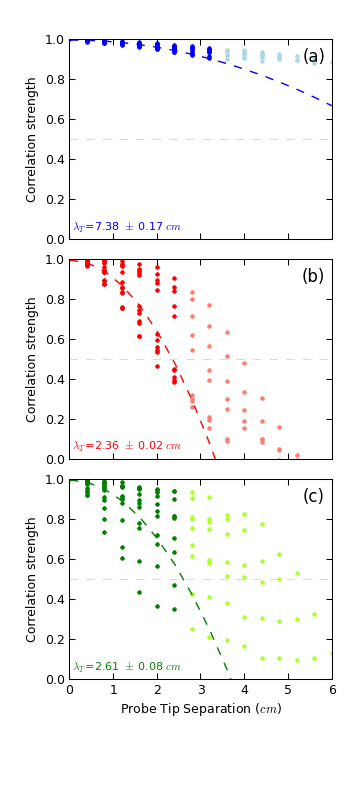
\includegraphics[width=8.5cm]{Images/brbtbz-081413.png}}
\caption{Single plume correlation functions for magnetic field in the (a) $\hat{r}$, (b) $\hat{\theta}$, (c) $\hat{z}$ directions}
\label{fig:brbtbz}
\end{figure}

Figure~\ref{fig:comparisons}(a) compares the spatial correlation functions from the single plume and colliding plume configurations of the experiment. The more narrow correlation function in the merging case is indicative of a more turbulent plasma and shorter correlation length. The parabolic fits are made to the first four points for each curve and the extracted Taylor scales also reflect the more narrow correlation function for  the merging case. Figure~\ref{fig:comparisons}(b) shows a comparison of the experimental single plume data to its single plume simulation counterpart. The shapes of the correlation functions are comparable within a few cm, but the simulation curve clear is steeper. The close correspondence at small separation distances results in a fairly close computed Taylor scale.

{\bf NB:} It's not clear to me why the Taylor scale in figure 3 is 3.3 cm for the single plume, but in figure 2, the Taylor scales are 2.36, 2.61, 7.38 cm.  It must be because different numbers of points used (looks like 6-8 points are used in figure 2, and only 4 in figure 3 maybe).  Also, the extrapolated lab single version down in figure 4 shows 2.06 cm.  That's the real one we want to report, I think.   Maybe a parabola with the real extrapolated Taylor scale should be used in figures 2 and 3?  Maybe figure 4 should come first?

Figure~\ref{fig:comparisons}(c) presents results from the merging configuration and its simulation counterpart. Unlike the single plume comparison, these two curves have distinctly different shapes; in addition, the simulation curve is broader than the experimental. This may be due the nature of the simulation at the midplane where the plumes are precisely meeting while it is not know exactly where the plumes meet in the experimental version. Using measurements slightly offset from the midplane of the simulation could imitate the variability in the merging plane of lab plasmas.

{\bf NB:} We need to revisit the simulation fits again.  Something isn't right.  Maybe the new higher res data will help.  Maybe we cut the simulation part.  I think just having the experimental results in figures 3 and 4 would be fine, i.e. just keeping 3a and the solid curves in 4.

\begin{figure}[!htbp]
\centering
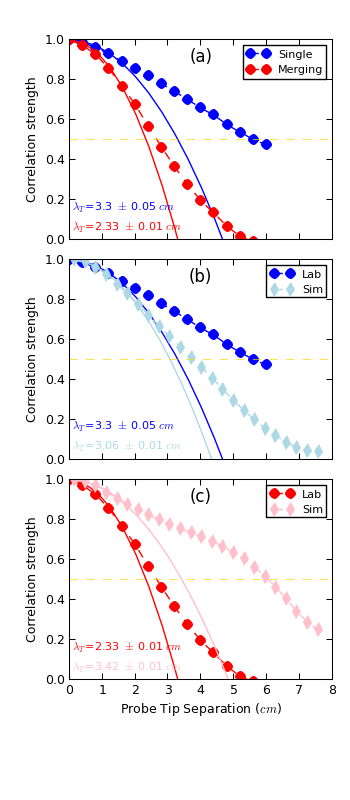
\includegraphics[width=8.5cm]{Images/comparisons.png}
\caption{\label{fig:comparisons} (a) Single vs.\ Merging. (b) Single, Lab vs.\ Sim. (c) Merging, Lab vs.\ Sim.}
\end{figure}

As shown in Figures \ref{fig:brbtbz} and \ref{fig:comparisons}, \eqref{eq:RM-eff} can be fit to correlation functions to obtain a value for the Taylor microscale $\lambda_T$. 
Following the example of Weygand et al. (which they call Richardson extrapolation) \cite{Weygand07}, we vary the number of points in the correlation function used in the fit and plot value of $\lambda_{T}$ extracted as a function of point number as shown in Fig.~\ref{fig:ndf}. Since the approximation for the Taylor microscale is calculated in the limit of zero-separation, the curves in Fig~\ref{fig:ndf} can be fit with a linear function in order to extrapolate the value of $\lambda_{T}$ at zero separation. We take this value of $\lambda_{T}$ as the best experimental value of the Taylor microscale.

\begin{figure}[!htbp]
\centerline{
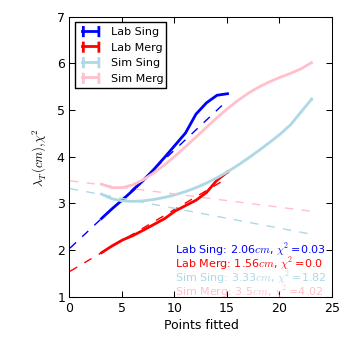
\includegraphics[width=0.5\textwidth]{Images/ndf.png}}
\caption{\label{fig:ndf} $\lambda_T$ vs. ndf. of parabola fit with error}
\end{figure}

Both the experimental single plume and colliding results show clear linearity in the trend. Fits to a linear function yield well-defined values of the Taylor microscale: $\lambda_T = 2.06~cm$ for the single plume configuration, and $\lambda_T = 1.56~cm$ for the merging setup. 

{\bf NB:} As noted above, we need to either figure out the simulation fits or just stick with the experimental result.

The simulation curves, however, do not have clearly linear trends. The trends in $\lambda_{T}$ appears to begin fairly linear for larger numbers of fit points, but begin to flatten and even slightly curve up as the number of fit points decreases. This is due to some flattening of the correlation function near zero. If the inflected portions of the lines are ignored, extrapolated values for zero-separation Taylor microscales appear to fall in the same range as the experiment. Note, however, that the single plume simulation appears to lie closer to the merging experiment than the single plume experiment. The overall merging correlation function also appears closer in shape to the single plume simulation. The merging simulation is the furthest again the furthest outlier.

Once the Richardson extrapolated $\lambda_T$ value has been obtained, calculating $R_{mT}$ can be computed using either of the values for $\lambda_{C}$ (integral scale $\lambda_{I}$ or energy-containing scale $\lambda_L$). Table~\ref{tab:Rms1} displays the Taylor microscale for each of the four datasets, along with the calculated Taylor Reynolds number computed using each form of $\lambda_{C}$. Note that the last column is consistent with the computed ``Spitzer'' Reynolds number using the energy-containing scale: $R_m = \mu_0 V \sigma_{SP} \lambda_L = 577$, but without the need to measure electron temperature or flow speed.

{\bf NB:} I don't understand table 2.  I think there's only one Spitzer Reynolds number to report.

\begin{table} [htbp]
\caption{\label{tab:Rms1}Comparison of Taylor Microscale and Taylor magnetic Reynolds numbers for various cases.}
\begin{tabular}{cccc}
\toprule
Dataset								& $\lambda_{T}$	&$R_{mT}(\lambda_{I})$&$R_{mT}(\lambda_L)$\\
\hline
Exp Single  					& 2.06 					& 7.8 								& 340\\					%
Sim Single  					& 2.38 					& 1.7 								& 255\\					%
Exp Merging 					& 1.56 					& 3.1 								& 593\\					%
Sim Merging 					& 2.62 					& 9.7 								& 210\\					%
\hline
\end{tabular}
\end{table}

{\bf NB:}  We'll need a new summary paragraph.

This paper presents a measurement of the magnetic spatial correlation function of an MHD turbulent plasma in a laboratory setting. Comparison of different types of plasma in the device shows that a single plume has a longer correlation length than merging plumes. The comparisons can be quantified by finding the zero-separation Taylor microscales for each plasma configuration which confirm the comparison of merging versus single plume. Moreover, the values found for the microscale are larger than any other expected dissipation scale; this is in line with the typical interpretation of the Taylor microscale in fluid physics. The Taylor microscale has in turn been used to compute Taylor magnetic Reynolds number. These values compare favorably to an estimate of the magnetic Reynolds number computed using Spitzer resistivity. Overall, the fact that the Reynolds number values are all $> 1$ show that the plasmas exhibit dissipation scales smaller than injection scales and likely have some (if short) inertial range physics. The method for measuring Taylor scales and Reynolds numbers in this way is shown to be applicable in an experimental device. Future work entails probing further how these scales change as plasma parameters are modified as well as much detailed comparison to space physics situations such as in the solar wind and the magnetosheath.

\section*{References}
\begin{thebibliography}{99}

\bibitem{Belmabrouk98}
H. Belmabrouk  and M. Michard, Taylor length scale measurement by laser Doppler velocimetry, Exp. Fluids {\bf 25}, 6976 (1998).

\bibitem{frisch95} U. Frisch, {\it Turbulence} (Cambridge: Cambridge Univ. Press) (1995).

\bibitem{Matthaeus05}
W. H. Matthaeus, S. Dasso, J. M. Weygand, L. J. Milano, C. W. Smith, and M. G. Kivelson, Phys. Rev. Lett. {\bf 95}, 231101 (2005). Spatial Correlation of Solar-Wind Turbulence from Two-Point Measurements

\bibitem{Weygand07}
J. M. Weygand, W. H. Matthaeus, S. Dasso, M. G. Kivelson, 
and R. J. Walker, J. Geophys. Res. {\bf 112}, A10201 (2007).

\bibitem{Weygand09}
J. M. Weygand, W. H. Matthaeus, S. Dasso, M. G. Kivelson, 
L. M. Kristler, and C. Mouikis, J. Geophys. Res. {\bf 114},
A07213 (2009).

\bibitem{Weygand10}
J. M. Weygand, W. H. Matthaeus, M. El-Alaoui, S. Dasso, and
M. G. Kivelson, J. Geophys. Res. {\bf 115}, A12250 (2010).

\bibitem{Weygand11}
J. M. Weygand, W. H. Matthaeus, S. Dasso, and M. G. Kivelson, J. Geophys. Res. {\bf 116}, A08120 (2011).

\bibitem{Matthaeus08}
W. H. Matthaeus, J. M. Weygand, P. Chuychai, S. Dasso, 
C. W. Smith, and M. Kivelson, Astrophys. J. {\bf 678},
L141 (2008).

\bibitem{Gray13} T. Gray, M. R. Brown, and D. Dandurand. Phys. Rev. Lett. {\bf 110}, 085002 (2013). 

\bibitem{Zhang11}
X. Zhang, D. Dandurand, T. Gray, M. R. Brown, and V. S. Lukin, ``Calibrated Cylindrical Mach Probe in a Plasma Wind Tunnel'', {\it Review of Scientific Instruments} {\bf 82}, 033510 (2011).

\bibitem{schaffner14a} D.A. Schaffner {\it et al.} Turbulence analysis of an experimental flux rope plasma. {\bf 56} 064003 (2014).

\bibitem{schaffner14b} 
D. Schaffner, A. Wan, and M. R. Brown, ``Observation of turbulent intermittency scaling with magnetic helicity in an MHD plasma wind-tunnel'', {\it Phys. Rev. Letters} {\bf 112}, 165001 (2014).

\end{thebibliography}

\end{document}

\begin{table} [htbp]
\caption{\label{tab:Rms2}Comparison of Taylor Microscale and Taylor magnetic Reynolds numbers for various cases.}
\begin{tabular}{ccccc}
\toprule
Dataset								&$R_{m}(\lambda_{I})$&$R_{m}(r_{1/2})$&$R_{m}(r_{wt})$&$R_{m}(\sigma_{SP})$\\
\hline
Exp Single  					& 60.3 								& 54.6						&200					&118-236\\
Sim Single  					& 2.84 								& 2.73						&112					&118-236\\
Exp Merging 					& 9.6 								& 10.4						&609					&118-236\\
Sim Merging 					& 93.6 								& 70							&76.5					&118-236\\
\hline
\end{tabular}
\end{table}

